\chapter{EPCglobal Architecture Framework}

\section{Overview}
\todo[inline]{Activities, Standards, Goals}

\section{Global Standardization}

\subsection{Importance}

\todo[inline]{The importance of a end-to-end architecture standard (enables comunication between every member in the value chain)}

\subsection{Efforts}

Standardization of \gls{UHF RFID} for item level tagging and \gls{supply chain}, by organizations like \gls{GS1}, provided a common language to identify, capture and share supply chain data, ensuring important information is accessible, accurate and easy to understand~\cite{anonymousStandardsGS12014}.

The first prominent adoption was by the \gls{DoD} with a policy released on July 30th 2004. The policy stated that contracts issued for material delivery would require the use of RFID tags. The policy was later extended to all commodities and commodities pallets shipped to any \gls{DoD} facility~\cite{DoDSuppliersPassive, DODReleasesFinal}.

In 2014, Impinj, Intel, Google and Smartrac, joined forces to create the \gls{RAIN RFID} alliance~\cite{TechnologyCompaniesCreate} after the ratification of \gls{GS1}'s \gls{UHF RFID} Generation 2 version 2 standard in November of 2013. The alliance promotes the universal adoption of \gls{GS1}'s Gen2 \gls{UHF RFID} technologies and the connection with \gls{cloud computing}, where RFID-based data can be stored, managed and shared via the Internet~\cite{WhatRAINRFID}.
The alliance fortified the adoption of \gls{GS1}'s standards and traced a common path for the the industry to progress.

On October 11th 2018 the European Commission published their positive implementation of the upper band in Europe~\cite{302208v030101pPdf}.
It extended the power levels to $2W$ in the lower band and added the requested global band from $915$MHz to $921$MHz with power levels up to $4W$. 
This was the biggest effort by the European Commission to establish a global standardized frequency band for \gls{UHF RFID} \gls{supply chain} applications.

\subsection{Current Problems}

There are still \gls{RFID} tags that do not conform with the international standards, often presenting proprietary formats and even encoding errors.
These closed practices and struggle for market supremacy around \gls{UHF RFID} creates a problematic situation that prevent conformity through the global logistics market.

Even in global standards, the adoption depends on the company and field of business. Usually one identification standard is already being used, and the migration cost for supporting multi-code integration can be high.

The information around global standards is also limited and hard to get through. It is divided in multiple specifications, identified with number notation and codification nomenclature. 
The ISO standards, in specific, are closed and have to be payed before even see it's contents.
These specifications are extensive and don't provide newcomers a good experience. 
Companies planning to implement \gls{UHF RFID} systems following legitimate global standardization resort to consultants who have a deep knowledge on the standards complexity.

The closed mentality in the area slowed the industry progression. In comparison with the cloud and web industries, where experience and software is shared and open-sourced, \gls{UHF RFID} tends to keep everything closed. The existent freely available software is old, outdated and out of maintenance. Experience from real-world implementations is unavailable making the industry prone to committing recurrent mistakes. This results in high investments in time and money on engineering resources that could be shared among industry leaders.

The positive implementation of the upper band frequency in Europe for global \gls{UHF RFID} \gls{supply chain} applications is also dependent on the acceptance by each European members. In particular, Germany and Netherlands are not accepting it~\cite{EUUpperBand}. The conflict with existing adopted bands in the countries makes a global homogeneous system a challenge that will need time to establish.

\section{GS1 and EPCglobal}

The GS1 is a nonprofit organization dedicated to the development and implementation of standards for global \gls{supply chain} solutions. 
The institution mission is to manage the GS1 System of Standards, create open, global, multi-sector standards fostering good business practices.

GS1 established itself in 2005 from the \gls{EAN} International, \gls{UCC} and other local organizations from the United States~\cite{PublicationLEBENSMITTELZEITUNGa}.
The organization took under its umbrella the former EAN-UCC roles subsuming their technologies. From those, worth mentioning: the barcode identification system (from \gls{EAN}), \gls{XML} standards, \gls{EDI} transaction sets and \gls{supply chain} solutions~\cite[p.~212]{lahiriRFIDSourcebook2005}.

The new GS1 organization then adopted much more ambitious projects, developing global standards and services for business communication.
From those efforts resulted the network for the synchronization of master data \gls{GDSN}, the \gls{EPC} integration for \gls{RFID}, traceability and the upstream integration of the consumer goods industry suppliers and EPCglobal Network.

For RFID Technology to become viable in practice, an infrastructure must exist for processing and communicating EPC data. In meeting the goal of creating a common infrastructure, MIT announced Auto-ID Release 1.0 in October 2003. At the same time, MIT entered into an exclusive licensing agreement with GS1.
In turn, GS1 established a new division called EPCglobal to implement Release 1.0 and to conduct further development based on industry input. This put forth an initial set of standards that formed the basis of an infra- structure for EPC data. Later, Auto-ID Release 1.0 became the starting-point for the EPCglobal Network~\cite[p. 50]{GlobalRFIDValue}. 
\todo[color=red, inline]{rewrite}

\todo[inline]{EPCglobal Spec history and context}

\section{Foundations and Technical Principles}

\todo[inline]{EPC Uniqueness, Identifiers, Decentralized Implementation, Issuing Organization, \dots}
\todo[inline]{Review text - it is from and ex subsection prior to the revision of the new index}

EPCglobal Architecture Framework is a collection of interrelated hardware, software, and data standards (\emph{EPCglobal Standards}) that interoperate with shared network services (\emph{EPC Network Services}) operated by GS1, its delegates, and others~\cite{Architecture6framework20140414Pdf}.

The existence of this standards promotes not only the global adoption of \gls{EPC}, but also the exchange of information between business partners. 

The fact that the \emph{EPCglobal Framework} only defines standards for interfaces and data, frees the market of \emph{information systems} to create custom business solutions. Manufacturing can have their custom business logic closed and expose production state information to the clients through the \emph{EPCglobal} standards.

The architecture establishes three core requirements and activities, all of which have a group of standards within the \emph{EPCglobal Architecture Framework}.

\paragraph{Physical Object Exchange} 

\emph{Identify} individual products, cases, loads, assets, return items, among others, so they can be tracked individually.
The \emph{End Users} parties in a supply chain that exchange physical objects that are identified with \gls{EPC}.
Physical object exchange consists in operations such as shipping, receiving goods, and so on.
For many End Users, the physical objects are trade goods, but this could not be the case.
There are many other uses, like library or asset management applications~\cite{dong-yingliDesignInternetThings2016} that differ from the \gls{supply chain} trade goods model, but still involve the requirement for unique identification and tagging of objects. 
The architecture must be designed to ensure that when one end user delivers a physical object to another end user, the latter will be able to determine the \gls{EPC} of the physical object and interpret it properly~\cite{Architecture6framework20140414Pdf}.
The \emph{EPCglobal Architecture Framework} defines \gls{EPC} physical object exchange standards.

\paragraph{Infrastructure for Data Capture} 

\emph{Capture data} about the movement of physical assets and creating visibility.
In order to have gather \gls{EPC} data, each \emph{End User} carries out operations within its environment. That can be the creation of \gls{EPC}s for new objects, follow the movements of objects by sensing their \gls{EPC}s, and gather that information into systems of record within the organization~\cite{Architecture6framework20140414Pdf}. The \emph{EPCglobal Architecture Framework} defines interface standards for the major infrastructure components required to gather and record \gls{EPC} data. This allows \emph{End Users} to develop their internal systems using interoperable components.

\paragraph{Data Sharing} 

\emph{Exchange data} with \gls{IT} applications and trading partners, to turn visibility into information and action.
\emph{End Users} benefit from the \emph{EPCglobal Architecture Framework} by sharing data with each other, increasing the visibility they have with respect to the movement of physical objects through the \gls{supply chain}. 
The \emph{EPCglobal Architecture Framework} defines \gls{EPC} data sharing standards, which provide a means for end users to share data about \gls{EPC}s within defined user groups or with the general public, and which also provide access to \emph{EPC Network Services} and other shared services that facilitate this sharing. \todo{change phrasing a bit}

\begin{figure}[!ht]
    \centering
    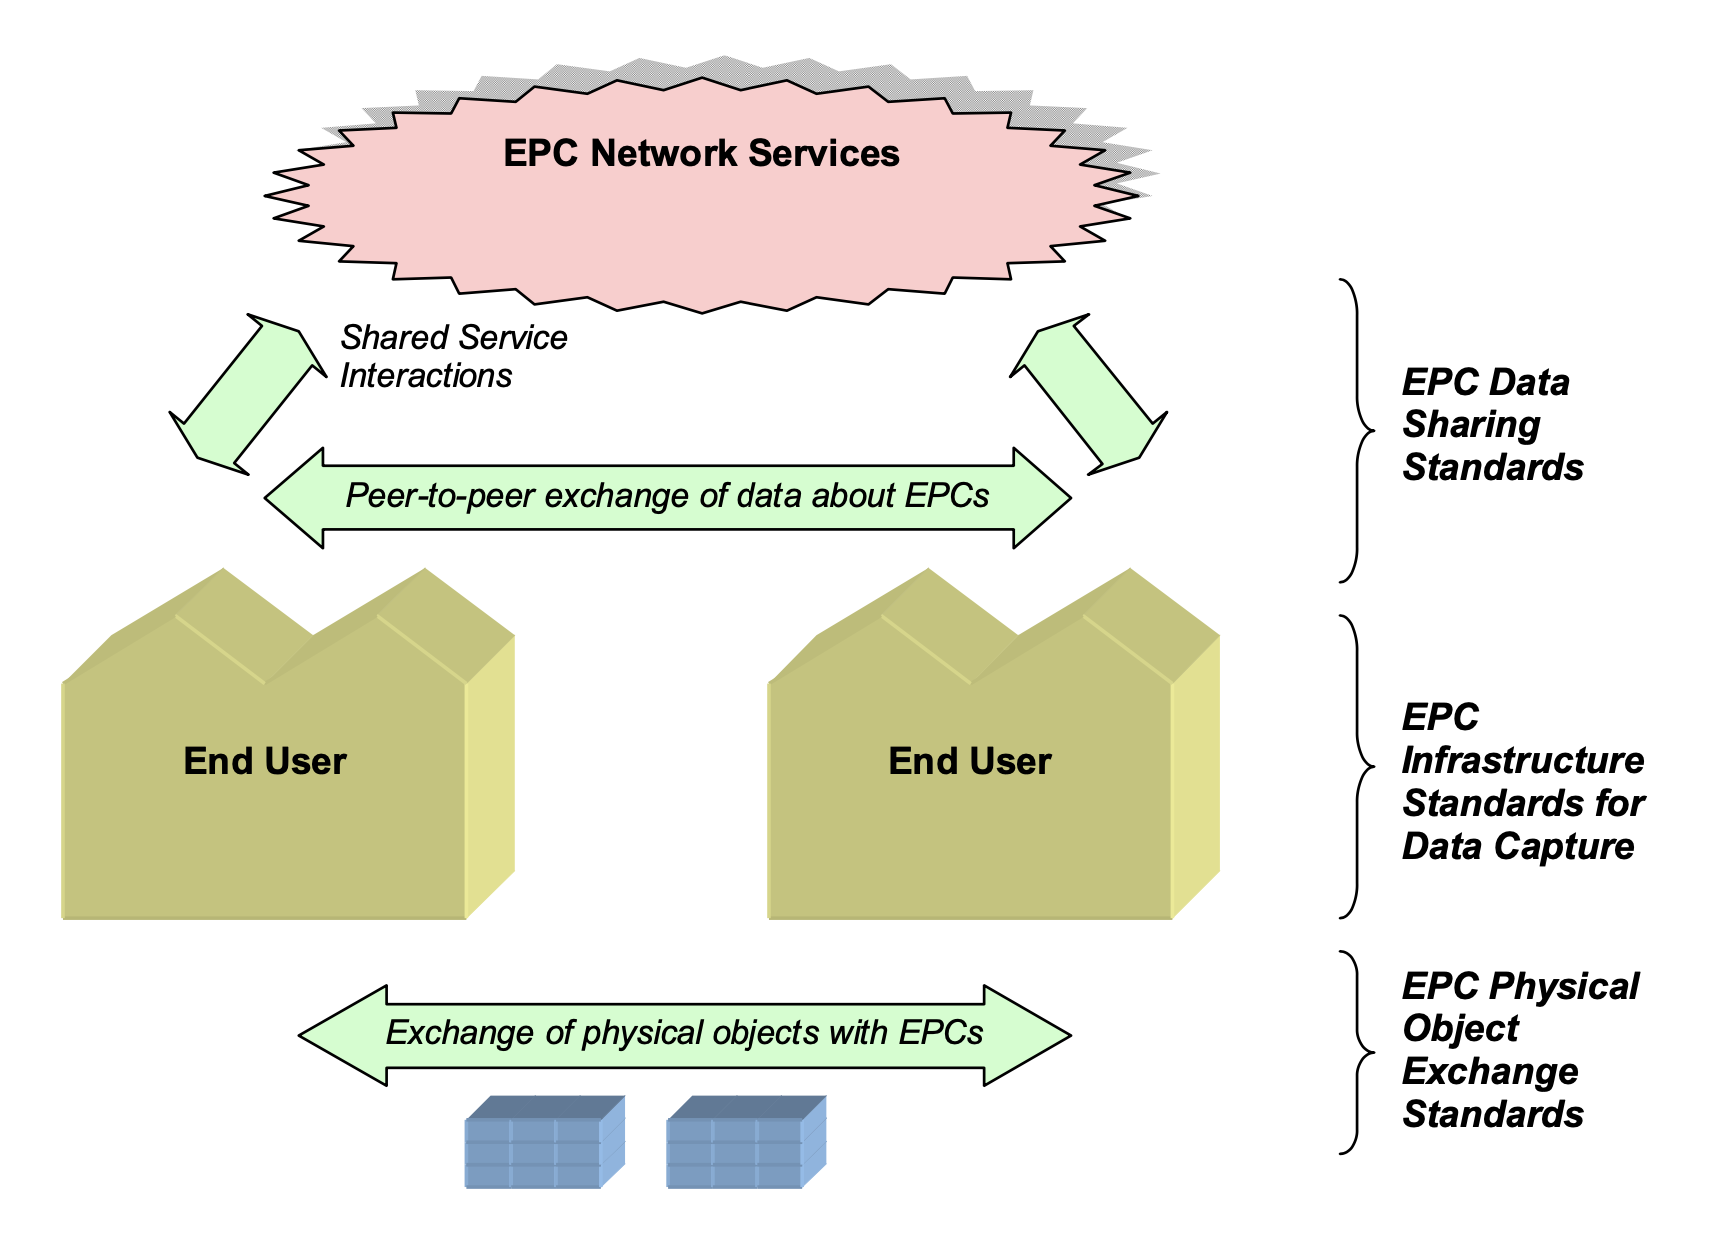
\includegraphics[width=0.9\textwidth]{./assets/02-state-of-the-art/architecture-framework-activities.png}
    \caption{\emph{EPCglobal Architecture Framework} activities~\cite{Architecture6framework20140414Pdf}} 
    \label{fig:02:architecture-activities}
\end{figure}

The \emph{EPCglobal Network} is a computer network used to share \gls{EPC} data between trading partners. 
It provides automatic, real-time identification and data sharing of items both within and outside of an company~\cite[p. 213]{lahiriRFIDSourcebook2005}.

Even doe the network was design mainly for \gls{RFID} sharing of \gls{EPC} data, the network does not exclusively runs on \gls{RFID} data carriers. The \emph{EPCglobal Network} can also be fed \gls{EPC} data through data carriers like 1D and 2D barcodes. The interoperability with the barcode was one of the most important considerations used during the planning of the network~\cite{RFIDBarcodeInteroperability}.

\todo[inline]{GS1 Architecture: organization, advantages and objectives: barcode inoperability}

\section{Dissertation Context}

\todo[inline]{What is relevant to the dissertation from the architecture framework, Roles, Interfaces and Standards used and why other things were left out, Outline of what will explained next}

\section{Tag Data Standard (TDS)}

\todo[inline]{C1G2 and ISO/IEC18000-6 Type C, Tag memory, EPC Structure, coding schemes and representations, GS1 keys relation, encoding of User memory and TID. Talk about Tag Data Translation (TDT). EPC interoperability with barcode.}

\todo[inline]{Check page 24 of the GS1 EPCglobal architecture Framework pdf}

\section{identification Key in Transport and Logistics}

\section{Filtering & Collection}

\subsection{Low Level Reader Protocol (LLRP)}

\gls{LLRP} is specification standard that defines an interface between \gls{RFID} Readers and \emph{Clients}.

Typically, an RFID system consists of network elements that participate in the management and transmission of tag data.
\emph{Client} network elements (e.g. end-user applications) are the consumers of this data.
The network elements between tag and \emph{Clients} form the road to transport tag data over the network to the applications, and convey tag operational commands over the network to tags.
The \gls{LLRP} interface specification is the standard that describes the communication between these network elements.


The interface recognizes that in some RFID systems, there is a requirement for RFID systems engineers, explicit knowledge of RFID air protocols, to tune the RFID air protocols. 
The coupling control of the physical layers of an RFID infrastructure may be useful for the purpose of mitigating RFID interference~\cite{Llrp1standard20101013Pdf}.
The \gls{LLRP} interface \emph{low-level} nature of the specification comes from this ability.

The responsibilities and requirements taken by the interface are:

\begin{itemize}
    \setlength{\parskip}{0pt}
    \setlength{\itemsep}{0pt}
    \item Proving means to command \gls{RFID} Readers to read, write inventory tags and perform other protocol-dependent commands as \emph{kill} and \emph{lock} from \emph{EPCglobal} \gls{C1G2};
    \item Give robust error and status report for tag access operations;
    \item Provide means for conveying tag passwords needed for protocol commands like \emph{kill} from \emph{EPCglobal} \gls{C1G2};
    \item Provide means to control and fetch information on the \gls{RF} link: power levels, spectrum utilization, estimation of \gls{RF} interference among Readers;
    \item Provide means to control parameters and aspects of the Tag Protocol operation;
    \item Been able to retrieve from Readers their capabilities;
    \item Provide means for ease addition of new air protocols;
    \item Support defining of vendor-specific extensions to the protocol from Reader devices vendors. Must be non-interfering  among vendors.
\end{itemize}

In the context of the \emph{EPCglobal} architecture framework, the elements relevant to the LLRP specification are the Tags, Readers and \gls{FC} Role.

\begin{figure}[!ht]
    \centering
    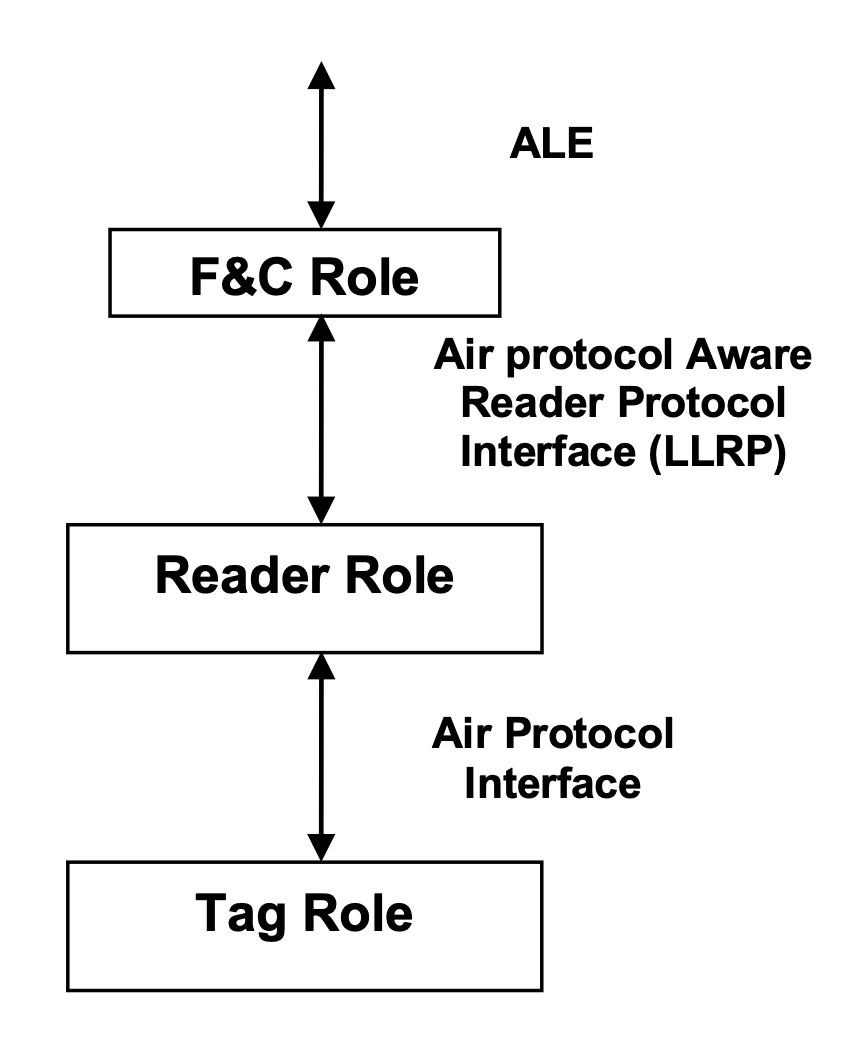
\includegraphics[width=0.4\textwidth]{./assets/02-state-of-the-art/llrp-interaction}
    \caption{\gls{LLRP} in the \emph{EPCglobal} Architecture~\cite{Llrp1standard20101013Pdf}} 
    \label{fig:02:llrp-interaction}
\end{figure}

\todo[inline]{Talk about LLRP for deployment of multiple readers e reader control and coordination?}

\section{Application Level Events (ALE)}

\section{EPCIS Capture Application}

\section{EPCIS Capture and Query Interfaces}

\section{EPCIS Repository}

\section{Core Business Vocabulary}

\section{Practical Context}

\todo[inline]{Nespresso supply-chain example and vision in the context of the EPCglobal framework, how it would work and advantages}